\chapter{Definitions}
A fundamental requirement of any information management system is the
protection of data and resources from unauthorized disclosure,
modification, or service denial, to ensure that the CIA properties are
sound. To achieve this, \textbf{access control} mechanisms ensure that
only authorized accesses occur within a system and to it's resources.

Access control is a major building block of network security,
regulating access of legitimate users to resources of a system, but by
itself, it cannot prevent the occurrence of cyber-attacks, nor
mitigate them, but like a firewall it uses rules to allow or deny
access to resources. However, effective protection schemes cannot
abstract from the definition of how access to system resources shall
take

\section{Definitions from Standards}
The concept of access control is formally defined in several standards:

\begin{itemize}
    \item \textbf{NISTIR 7298}: Access control is "the process of
      granting or denying specific requests to obtain and use
      information and related information processing services, or to
      enter specific physical facilities (\textit{which we will not
      deal with in this course})."
    \item \textbf{RFC 4949}: Access control is "a process by which use
      of system resources is regulated according to a security policy
      and is permitted only by authorized entities (users, programs,
      processes, or other systems)."
\end{itemize}

\section{Access Control Security Requirements}
Access control mechanisms should allow specification of:

\begin{enumerate}
    \item Authorized users and their permissions.
    \item The resources they can access.
    \item The duration and conditions of access.
    \item The specific operations they are permitted to perform.
\end{enumerate}

A comprehensive set of security requirements is outlined in NIST SP
800-171, including:

\paragraph{Basic Security Requirements}
\begin{enumerate}
    \item Restrict system access to authorized users, processes, and devices.
    \item Limit user access to only authorized transactions and functions.
\end{enumerate}

\paragraph{Derived Security Requirements}

\begin{enumerate}
    \item Enforcement of information flow restrictions in accordance
      to the policies.
    \item Separation of duties to prevent collusion.
    \item Implementation of the principle of least privilege.
    \item Prevention of non-privileged users from executing privileged
      functions.
      \subitem The system must perform authorization checks will still
      ensuring that the privacy of the user is maintained.
    \item Limit unsuccessful logon attempts.
    \item Use of cryptographic mechanisms for securing remote access.
    \item Authorization and encryption for wireless access.
    \item Control over external system connections and mobile devices.
    \item Terminate a user session after some conditions or period of
      inactivity.
\end{enumerate}

The NIST mapped all the possible scenarios, the first 3 are the most
important, but it's important that as many possible scenarios are
mapped to ensure that the system is secure.

\section{Access Control Principles}
Access control is a core aspect of computer security, as such it's
important to follow well established guidelines. RFC 4949 defines
computer security as "measures that implement and assure security
services in a computer system, particularly those that assure access
control service."

\begin{figure}[H]
  \centering
  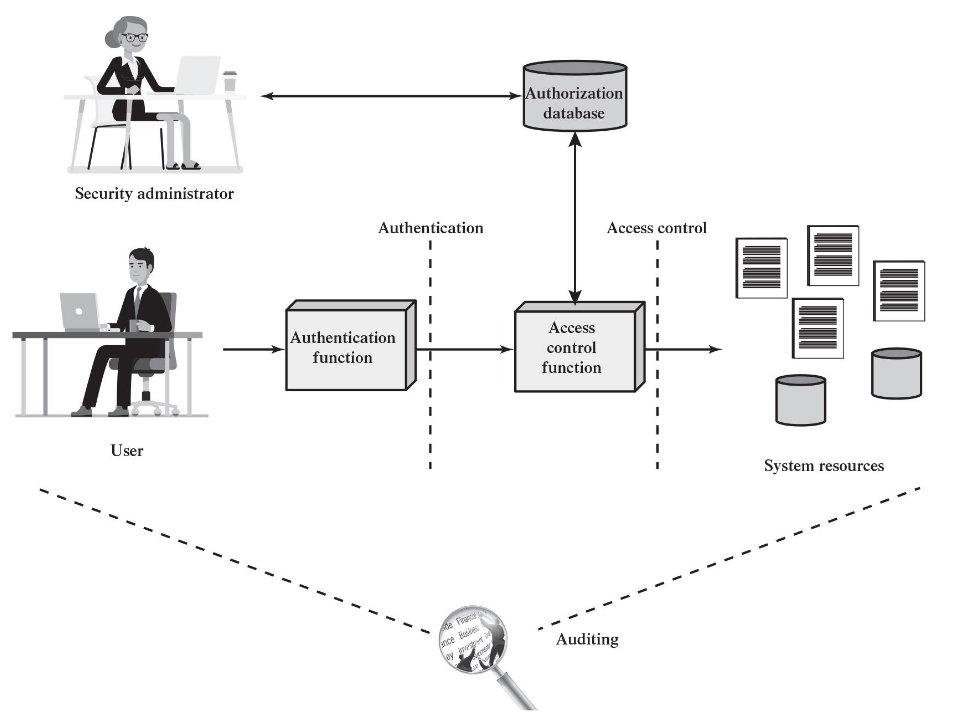
\includegraphics[width=0.4\textwidth]{img/Access Control Principles.png}
  \caption{Access Control Schema in brief}
\end{figure}


\section{Relationship with Other Security Functions}
Access control interacts with several other security functions, which
occurs at different stages of the security process:

\begin{enumerate}
    \item \textbf{Authentication}: Verifies user credentials before
      granting access.
    \item \textbf{Authorization}: Determines permissions based on
      policies and trust levels. This function determines who is
      trusted for a given purpose.
    \item \textbf{Audit}: Verifies that the policies of the company
      are fully implemented and that the access control mechanisms are
      working as expected.
  \end{enumerate}

In this scenario, there are different actors. The user accesses the
systems resources after being authenticated by the authentication
function The security administrators manage an authorization database,
while authentication functions verify users before granting access.
Auditing provides an independent review to maintain security
compliance.

\section{Authentication and Audit}
Authentication ensures that a user or process is verified before accessing
system resources. Auditing plays a crucial role in maintaining security by
monitoring activities.

\subsection{Internal and External Audit}
IT enterprises conduct two types of audits:

\textbf{Internal Audit} is performed within the organization to identify risks
related to performance, security, and compliance. Internal auditors monitor
mitigation efforts to improve the organization’s security posture.

\textbf{External Audit} is conducted by independent professionals, often
Certified Public Accountants (CPAs), who assess an organization's security and
compliance. External audit reports are vital for stakeholders and
clients, and generally comes with some kind of certification granted
by a third party.

\begin{figure}[h]
  \centering
  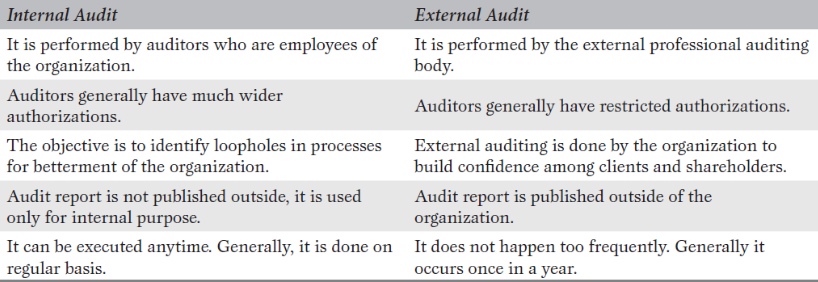
\includegraphics[width=0.7\textwidth]{img/internal-external-audit.png}
  \caption{Internal and External Audit}
\end{figure}

Keep in mind that when we refer to auditing, cyber security auditing,
of course, we can not only analyze the access control procedures, but
also other aspects, like the security computer, the network security
configuration, the software security computation, and so on. All these 
aspects can provide a feedback to improve the authorization database 
and the access control mechanisms.

\section{Access Control Mechanisms}
\begin{boxH}
  An access control mechanism \textbf{regulates interactions} between
  users and system resources (applications, files, databases, etc.).
\end{boxH}

The process of access control begins with user authentication, which
verifies the identity of the user requesting access to a specific
resource. Once authenticated, the system determines the user's
permissions and privileges, taking into account the policies specified
by security administrators. This information is stored in an
authorization database that maps user identities to resources and
services.

The access control function relies on this database to make decisions
about granting or denying requests. While this is a straightforward
scheme, there are complexities to consider. For instance, coordinating
multiple databases and technologies can be challenging, especially for
small organizations with limited resources.

In many cases, security administrators must configure each
authorization mechanism individually, which can lead to
inconsistencies and difficulties in maintaining coherence across the
system. Furthermore, as businesses increasingly rely on cloud
providers like Amazon, the need for a unified electronic access
mechanism (EAM) becomes crucial.

In some scenarios, there may not be a single EAM that can coordinate
all authorization mechanisms, leading to fragmentation and potential
security risks. However, this is where the coordination with the
database comes into play – the security administrator specifies the
policy in one unique point, which all other components must adhere to.

Operating systems incorporate built-in access control functions,
supplemented by security add-ons and application-specific controls.
External devices, such as firewall, can also provide access control
services, which is different from the access control on the users. 

All those ideas are then conveyed in three main concepts:
\begin{itemize}
  \item Security mechanism
  \item Security policy
  \item Security model
\end{itemize}
\subsection{Security Mechanisms}
Security mechanisms enforce policies, which are defined trough the
policies and formally stated by the model, through software and
hardware functions.

\subsection{Access Control Policies}
Access control policies define high level rules for regulating user
access. They specify what types of access are permitted, under what
conditions, and by whom. These policies can be formalized into
\textbf{authorization databases}.

\subsubsection{Separation between mechanism and policy}
As for every high-level/low-level separation, the separation between
mechanism and policy allows to define the implementation of the system
indipendetly of the protection requirements. 
It is also possible to compare different access control policies as
well as  different mechanisms that enforce the same policy.

One of the most important aspects is the possibility to design
mechanisms that enforce multiple policies: if a mechanism is designed
to enforce a single policy and be tied to it, a change in the policy
would require changing the whole access control system.

\subsection{Access Control Policy Model}
It provides a formal representation of the access control security
policy and its working. The formalization allows the proof of
properties on the security provided by the access control system being
designed.

\section{Subjects, Objects, and Access Rights}
Typically, a specific policy is characterized by the concepts of
subjects, objects, and access rights, or at least Discretionary Access
Control (DAC) and Role-Based Access Control (RBAC) are.

\textbf{Objects} include files, databases, messages, and programs. The number
and type of protected objects depend on system complexity and security
requirements.

\textbf{Subjects} represent active entities such as users, applications, and
processes. Subjects are accountable for their actions, with audit trails
recording relevant activities.

\textbf{Actions} refer to access operations on objects form subjects
that have access rights, such as Read, Write, Execute, Delete, Create,
and Search. Read access includes the ability to copy or print, while
write access includes read access.

\section{Access Control Policy Models}
Access control policies are categorized into:

\textbf{Discretionary Access Control (DAC)}: Grants access based on user
identity and explicit authorization rules. Users can delegate their access
privileges to others.

\textbf{Mandatory Access Control (MAC)}: Enforces access restrictions based on
security labels and clearance levels. Users cannot override these restrictions.

\textbf{Role-Based Access Control (RBAC)}: Grants access based on
organizational roles rather than individual identities. Users inherit
permissions from their assigned roles.

\textbf{Attribute-Based Access Control (ABAC)}: Grants access based on
attributes of users, objects, and environmental conditions, offering a flexible
and dynamic approach.

These four policies are not mutually exclusive. An access control
mechanism may employ two or even all three of these policies to cover
different classes of system resources.

\subsection{Discretionary Access Control (DAC)}
\begin{boxH}
  Discretionary policies enforce access control on the basis of the
  \textbf{identity} of the requestors and \textbf{explicit access
  rules} that establish who can, or cannot, execute which actions on
  which resources.
\end{boxH}
Usually, this kind of policy is expressed by an access matrix, like
the one in figure \ref{fig:access-matrix}. The rows represent the 
subjects, the columns the objects, and the cells the access rights of 
the subjects on the objects.

\begin{figure}[H]
  \centering
  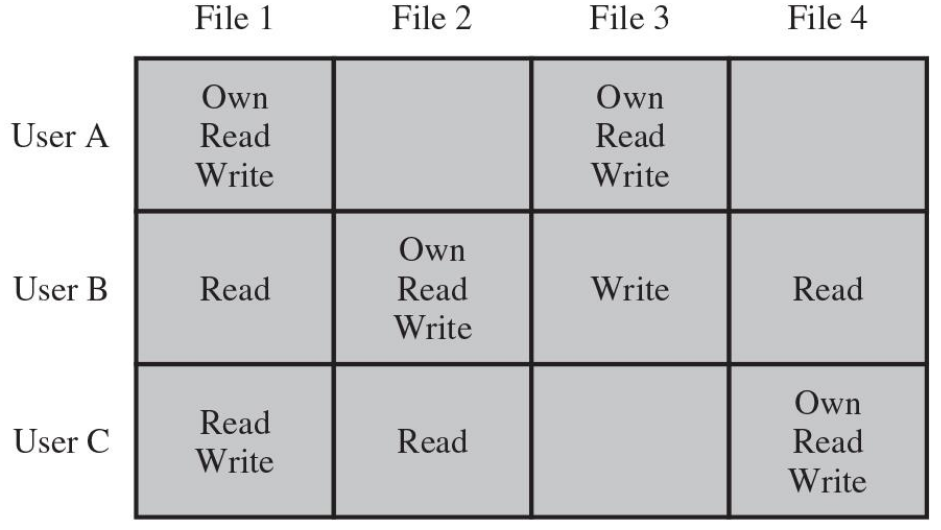
\includegraphics[width=0.5\textwidth]{img/access matrix.png}
  \caption{Access Matrix}
  \label{fig:access-matrix}
\end{figure}
This matrix is a simple way to represent the access control policy, 
but not a good way to implement it. The matrix is sparse(there could
be many empty cells), and it is not efficient to store it in memory,
without even considering the management of the redundancy of the 
information.

For a more practical approch there are 3 different alternatives.
\subsubsection{Authorization Tables}
Authorization tables are a more efficient way to represent access
control policies. They store access rules in a more compact way,
without leaving empty cells, like in figure \ref{fig:auth-table}.

\begin{figure}[H]
  \centering
  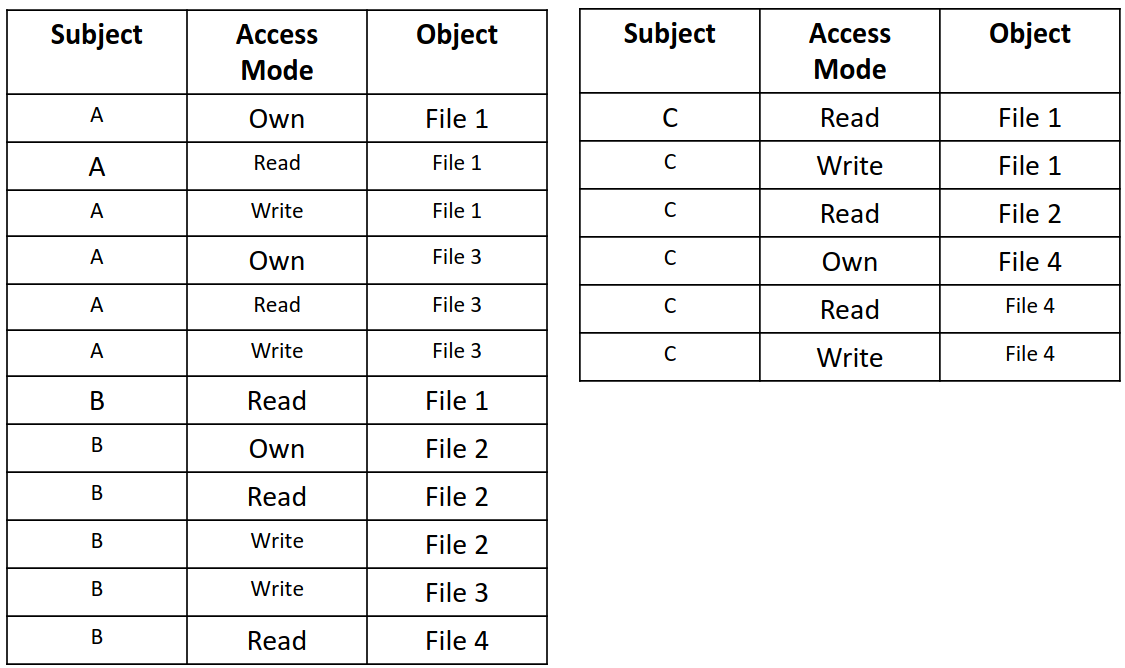
\includegraphics[width=0.6\textwidth]{img/auth table.png}
  \caption{Authorization Table}
  \label{fig:auth-table}
\end{figure}

It's possible to further reduce the redundancy of the data by
splitting the column in different table and using join operations to
reconstruct the original table if needed.

\subsubsection{Access Control Lists (ACLs) and Capability Lists}
With an Access Control List (ACL), each object has a list of users and
their access rights. This list is stored in the object's metadata, and
is checked whenever a user requests access to the object.

A similar concept is the Capability List, where each user has a list
of objects and their access rights.

\begin{figure}[H]
  \centering
  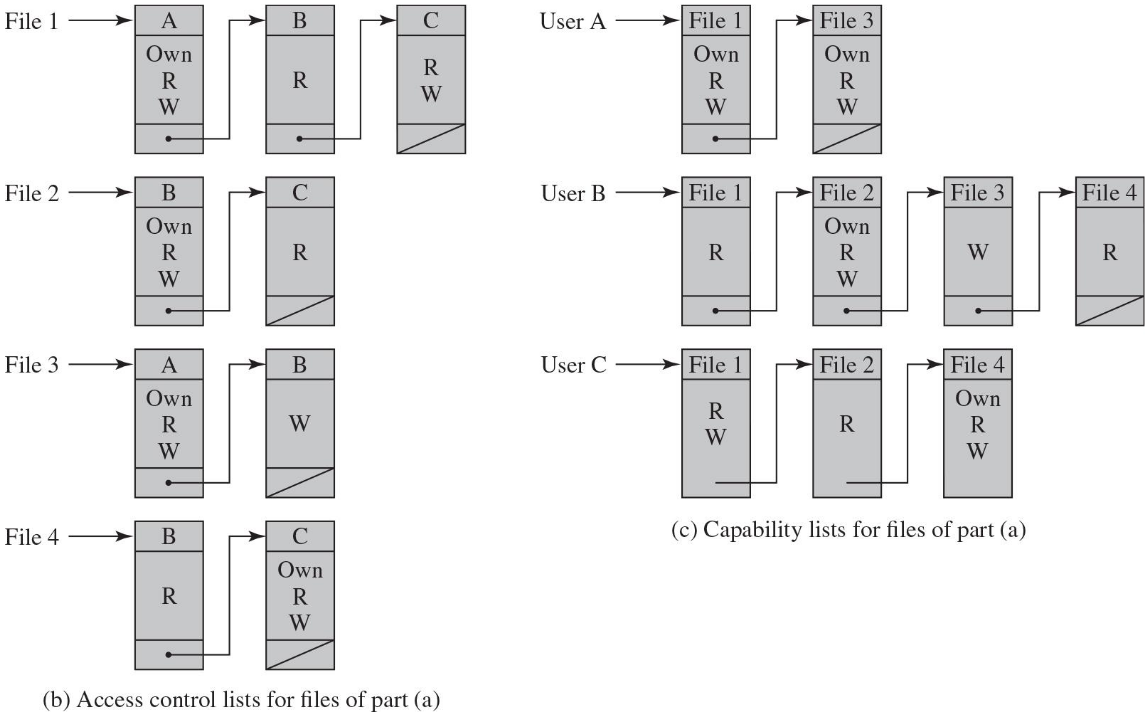
\includegraphics[width=0.6\textwidth]{img/acl.png}
  \caption{Access Control List}
  \label{fig:acl}
\end{figure}

\subsection{Mandatory Access Control (MAC)}
Mandatory Access Control (MAC) policies are based on \textbf{security
labels} (which indicate the sensitivity or criticality of the
information/resource) and \textbf{clearance levels}, or security
permission, which are assigned to subjects and indicate that the
subject can access the resources.

Mandatory Access Control was originally introduced in critical
domains, like military-grade once, but DAC has become more prevalent
nowadays, even though this model is more maintainable.
The logic is shown in figure \ref{fig:mac}.
The administrator specifies the confidential level of the data, define
define which users are allowed to access on specific level of
confidentiality and security, and the system will enforce the policy.

\begin{figure}[H]
  \centering
  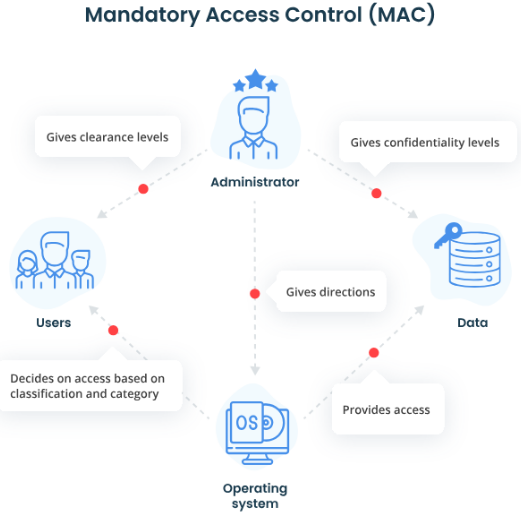
\includegraphics[width=0.4\textwidth]{img/mac.png}
  \caption{Mandatory Access Control}
  \label{fig:mac}
\end{figure}

\subsection{Role-Based Access Control (RBAC)}

Role-based access control (RBAC) is an alternative to traditional
discretionary (DAC) and mandatory access control (MAC) policies that
is attracting increasing attention, particularly for commercial
applications.



RBAC is designed to enforce security policies that align with an
organization’s structure. In many business environments, a user’s
identity is primarily relevant for accountability purposes, while
access control decisions are better based on the user’s organizational
responsibilities rather than their individual identity.

Traditional DAC, which emphasize user ownership of data, often do not
fit well in enterprise settings. Similarly, MAC, where users have
security clearances and objects have security classifications, can be
too rigid. RBAC addresses this gap by combining explicit authorization
mechanisms with organizational constraints, providing a balance
between flexibility and structured access control.

Unlike DAC systems, which define access rights for individual users
and groups, RBAC revolves around roles. A role in RBAC represents a
job function within the organization, and access rights are assigned
to these roles instead of directly to users. Users are then assigned
roles, either statically or dynamically, based on their
responsibilities, ensuring a more scalable and manageable approach to
access control.

\section{Implementation of Access Control}
Access control mechanisms are implemented using:

- \textbf{Access Control Lists (ACLs)}: Define permissions for each user-object
pair.
- \textbf{Capability Lists}: Assign access rights to subjects rather than
objects.
- \textbf{Authorization Tables}: Store access rules as a set of conditions.

\section{Advanced Access Control Concepts}
\subsection{Least Privilege and Separation of Privilege}
The principle of least privilege ensures that subjects are granted the minimum
access necessary to perform their tasks, reducing the risk of unauthorized
actions.

Separation of privilege divides access across multiple entities, requiring more
than one authorization to perform critical actions, thereby mitigating insider
threats.

\subsection{Role Hierarchies and Constraints in RBAC}
Role hierarchies allow roles to inherit permissions from superior roles.
Constraints define conditions such as:

- Mutually exclusive roles (a user can hold only one role in a set).
- Cardinality limits (restricting the number of users per role).
- Prerequisite roles (requiring users to hold a specific role before obtaining
another).

\subsection{ABAC and its Flexibility}
ABAC offers a powerful and flexible access control model by evaluating
attributes of subjects, objects, and environmental conditions. However, it
requires high computational effort, making it more complex than DAC and RBAC.

